% !TEX program = pdflatex
\documentclass[aspectratio=169]{beamer}
\usetheme{Madrid}
\usecolortheme{default}
\usepackage{tikz}

% Custom colors
\definecolor{myblue}{RGB}{0,114,178}
\definecolor{myorange}{RGB}{230,159,0}
\definecolor{mygreen}{RGB}{0,158,115}
\definecolor{myred}{RGB}{213,94,0}
\definecolor{mypurple}{RGB}{204,121,167}
\definecolor{mybrown}{RGB}{240,228,66}
\definecolor{mygray}{RGB}{189,189,189}

% Set colors
\setbeamercolor{title}{fg=white,bg=myblue}
\setbeamercolor{frametitle}{fg=white,bg=myblue}
\setbeamercolor{section title}{fg=white,bg=myblue}
\setbeamercolor{subsection title}{fg=white,bg=myorange}
\setbeamercolor{item}{fg=myblue}
\setbeamercolor{subitem}{fg=myorange}

% Remove navigation symbols
\setbeamertemplate{navigation symbols}{}

% Title page
\title{Numerical Methods}
\subtitle{Newton's Method and Euler's Method}
\author{Differential Calculus}
\date{}

\begin{document}

\begin{frame}
\titlepage
\end{frame}

\begin{frame}{Outline}
\tableofcontents
\end{frame}

\section{Introduction}

\begin{frame}{Why Numerical Methods?}
\begin{itemize}
    \item Many mathematical problems cannot be solved exactly using analytical methods
    \item Numerical methods provide approximate solutions using iterative procedures
    \item These methods are essential in:
    \begin{itemize}
        \item Engineering and physics simulations
        \item Financial modeling and optimization
        \item Computer graphics and animation
        \item Scientific computing and data analysis
    \end{itemize}
    \item Two fundamental methods: Newton's Method and Euler's Method
\end{itemize}
\end{frame}

\section{Newton's Method}

\begin{frame}{Newton's Method - Introduction}
\begin{itemize}
    \item Newton's Method is used to find roots of equations: $f(x) = 0$
    \item It's an iterative method that uses linear approximation
    \item Based on the idea: if we have a good guess $x_n$, we can get a better guess $x_{n+1}$
    \item Uses the tangent line to approximate where the function crosses the x-axis
    \item Very fast convergence for most functions
\end{itemize}
\end{frame}

\begin{frame}{Newton's Method - Geometric Intuition}
\begin{center}
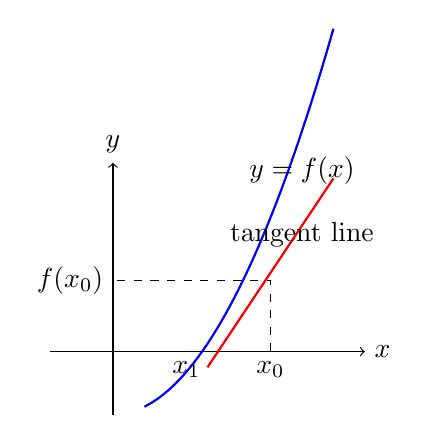
\begin{tikzpicture}[scale=0.8]
\draw[->] (-1,0) -- (4,0) node[right] {$x$};
\draw[->] (0,-1) -- (0,3) node[above] {$y$};
\draw[domain=0.5:3.5, smooth, variable=\x, blue, thick] plot ({\x}, {0.5*\x*\x - 1});
\draw[domain=1.5:3.5, smooth, variable=\x, red, thick] plot ({\x}, {1.25 + 1.5*(\x-2.5)});
\draw[dashed] (2.5,0) -- (2.5,1.125) -- (0,1.125);
\draw[dashed] (1.167,0) -- (1.167,0) -- (0,0);
\node[below] at (2.5,0) {$x_0$};
\node[below] at (1.167,0) {$x_1$};
\node[left] at (0,1.125) {$f(x_0)$};
\node[above] at (3,2.5) {$y = f(x)$};
\node[above] at (3,1.5) {tangent line};
\end{tikzpicture}
\end{center}

\textbf{Key Elements:}
\begin{itemize}
    \item Blue curve: $y = f(x)$ (the function we want to find roots of)
    \item Red line: tangent line at point $(x_0, f(x_0))$
    \item $x_0$: our initial guess
    \item $x_1$: where tangent line crosses x-axis (next guess)
    \item $f(x_0)$: function value at our initial guess
\end{itemize}
\end{frame}

\begin{frame}{Newton's Method - Step-by-Step Process}
\textbf{The Newton's Method Process:}
\begin{enumerate}
    \item Start with initial guess $x_0$
    \item Draw tangent line at point $(x_0, f(x_0))$
    \item Find where tangent line crosses x-axis: $x_1$
    \item Use $x_1$ as new guess and repeat process
    \item Continue until convergence
\end{enumerate}

\vspace{0.5cm}
\textbf{Why This Works:}
\begin{itemize}
    \item Tangent line is a good approximation of $f(x)$ near $x_0$
    \item Where tangent crosses x-axis is close to where $f(x)$ crosses x-axis
    \item Each iteration gets us closer to the actual root
    \item Process converges very quickly (quadratic convergence)
\end{itemize}

\vspace{0.5cm}
\textbf{Mathematical Insight:}
\begin{itemize}
    \item Tangent line equation: $y = f(x_0) + f'(x_0)(x - x_0)$
    \item Set $y = 0$ to find where it crosses x-axis
    \item Solve: $0 = f(x_0) + f'(x_0)(x_1 - x_0)$
    \item Result: $x_1 = x_0 - \frac{f(x_0)}{f'(x_0)}$
\end{itemize}
\end{frame}

\begin{frame}{Newton's Method - Derivation}
\textbf{Step-by-step derivation:}
\begin{itemize}
    \item We have a guess $x_n$ and want to find a better guess $x_{n+1}$
    \item The tangent line at $(x_n, f(x_n))$ has equation:
    \[y = f(x_n) + f'(x_n)(x - x_n)\]
    \item This line crosses the x-axis when $y = 0$:
    \[0 = f(x_n) + f'(x_n)(x_{n+1} - x_n)\]
    \item Solving for $x_{n+1}$:
    \[x_{n+1} = x_n - \frac{f(x_n)}{f'(x_n)}\]
\end{itemize}
\end{frame}

\begin{frame}{Newton's Method - Formula}
\textbf{Newton's Method Formula:}
\[x_{n+1} = x_n - \frac{f(x_n)}{f'(x_n)}\]

\textbf{Key Points:}
\begin{itemize}
    \item Requires both $f(x)$ and $f'(x)$
    \item Need a good initial guess $x_0$
    \item Method fails if $f'(x_n) = 0$ (horizontal tangent)
    \item Usually converges very quickly (quadratic convergence)
    \item Stop when $|x_{n+1} - x_n| < \epsilon$ or $|f(x_n)| < \epsilon$
\end{itemize}
\end{frame}

\begin{frame}{Newton's Method - Detailed Derivation}
\textbf{Complete Mathematical Derivation:}
\begin{itemize}
    \item Start with initial guess $x_1$ for solution of $f(x) = 0$
    \item Tangent line at $x = x_1$: $y = F(x) = f(x_1) + f'(x_1)(x - x_1)$
    \item Solve $F(x) = 0$ for $x_2$:
    \[0 = f(x_1) + f'(x_1)(x_2 - x_1)\]
    \[x_2 - x_1 = -\frac{f(x_1)}{f'(x_1)}\]
    \[x_2 = x_1 - \frac{f(x_1)}{f'(x_1)}\]
    \item Repeat: $x_{n+1} = x_n - \frac{f(x_n)}{f'(x_n)}$
\end{itemize}
\end{frame}

\begin{frame}{Newton's Method - Algorithm}
\textbf{Newton's Method Algorithm:}
\begin{enumerate}
    \item Make a preliminary guess $x_1$
    \item Define $x_2 = x_1 - \frac{f(x_1)}{f'(x_1)}$
    \item Iterate: for each natural number $n$, once you have computed $x_n$, define
    \[x_{n+1} = x_n - \frac{f(x_n)}{f'(x_n)}\]
    \item Stop when $|x_{n+1} - x_n| < \epsilon$ or $|f(x_n)| < \epsilon$
\end{enumerate}
\end{frame}

\begin{frame}{Example 1: Newton's Method for Square Root}
\textbf{Problem:} Use Newton's Method to approximate $\sqrt{5}$

\textbf{Think about:}
\begin{itemize}
    \item What equation has $\sqrt{5}$ as a solution?
    \item What function should you use?
    \item What is a good initial guess?
    \item What is the derivative of your function?
\end{itemize}
\end{frame}

\begin{frame}{Example 1: Newton's Method for Square Root - Solution}
\textbf{Solution:}
\begin{itemize}
    \item We want to solve $x^2 = 5$, so $f(x) = x^2 - 5$
    \item $f'(x) = 2x$
    \item Choose initial guess: $x_0 = 2$ (close to $\sqrt{5} \approx 2.236$)
    \item Newton's formula: $x_{n+1} = x_n - \frac{x_n^2 - 5}{2x_n} = \frac{x_n + \frac{5}{x_n}}{2}$
\end{itemize}
\end{frame}

\begin{frame}{Example 1: Newton's Method for Square Root - Solution (Continued)}
\textbf{Iterations:}
\begin{itemize}
    \item $x_0 = 2$
    \item $x_1 = \frac{2 + \frac{5}{2}}{2} = \frac{2 + 2.5}{2} = 2.25$
    \item $x_2 = \frac{2.25 + \frac{5}{2.25}}{2} = \frac{2.25 + 2.222...}{2} = 2.2361$
    \item $x_3 = \frac{2.2361 + \frac{5}{2.2361}}{2} = 2.236068$
    \item Actual value: $\sqrt{5} = 2.236068...$
    \item Very fast convergence!
\end{itemize}
\end{frame}

\begin{frame}{Example 2: Newton's Method for Equation Solving}
\textbf{Problem:} Use Newton's Method to find a root of $f(x) = x^3 - 2x - 5$

\textbf{Think about:}
\begin{itemize}
    \item What is the derivative of this function?
    \item What would be a good initial guess?
    \item How can you check if your answer is reasonable?
\end{itemize}
\end{frame}

\begin{frame}{Example 2: Newton's Method for Equation Solving - Solution}
\textbf{Solution:}
\begin{itemize}
    \item $f(x) = x^3 - 2x - 5$
    \item $f'(x) = 3x^2 - 2$
    \item Newton's formula: $x_{n+1} = x_n - \frac{x_n^3 - 2x_n - 5}{3x_n^2 - 2}$
    \item Choose initial guess: $x_0 = 2$ (since $f(2) = 8 - 4 - 5 = -1$ and $f(3) = 27 - 6 - 5 = 16$)
\end{itemize}
\end{frame}

\begin{frame}{Example 2: Newton's Method for Equation Solving - Solution (Continued)}
\textbf{Iterations:}
\begin{itemize}
    \item $x_0 = 2$
    \item $x_1 = 2 - \frac{8 - 4 - 5}{12 - 2} = 2 - \frac{-1}{10} = 2.1$
    \item $x_2 = 2.1 - \frac{9.261 - 4.2 - 5}{13.23 - 2} = 2.1 - \frac{0.061}{11.23} = 2.0946$
    \item $x_3 = 2.0946 - \frac{9.19 - 4.189 - 5}{13.16 - 2} = 2.0946 - \frac{0.001}{11.16} = 2.0945$
    \item Check: $f(2.0945) = 9.19 - 4.189 - 5 = 0.001$ (very close to 0)
\end{itemize}
\end{frame}

\begin{frame}{Example 3: Approximating $\sqrt{2}$}
\textbf{Problem:} Use Newton's Method to approximate $\sqrt{2}$

\textbf{Solution:}
\begin{itemize}
    \item Solve $f(x) = x^2 - 2 = 0$
    \item $f'(x) = 2x$
    \item Newton's formula: $x_{n+1} = x_n - \frac{x_n^2 - 2}{2x_n} = \frac{x_n}{2} + \frac{1}{x_n}$
    \item Start with $x_1 = 1.5$ (between 1 and 2)
\end{itemize}
\end{frame}

\begin{frame}{Example 3: Approximating $\sqrt{2}$ - Iterations}
\textbf{Detailed Iterations:}
\begin{itemize}
    \item $x_1 = 1.5$
    \item $x_2 = \frac{1.5}{2} + \frac{1}{1.5} = 0.75 + 0.6667 = 1.416666667$
    \item $x_3 = \frac{1.416666667}{2} + \frac{1}{1.416666667} = 0.7083 + 0.7059 = 1.414215686$
    \item $x_4 = \frac{1.414215686}{2} + \frac{1}{1.414215686} = 0.7071 + 0.7071 = 1.414213562$
    \item $x_5 = \frac{1.414213562}{2} + \frac{1}{1.414213562} = 1.414213562$
    \item $\sqrt{2} \approx 1.414213562$ (9 decimal places accuracy!)
\end{itemize}
\end{frame}

\begin{frame}{Example 4: Approximating $\pi$}
\textbf{Problem:} Use Newton's Method to approximate $\pi$

\textbf{Solution:}
\begin{itemize}
    \item Solve $f(x) = \sin(x) = 0$ (since $\sin(\pi) = 0$)
    \item $f'(x) = \cos(x)$
    \item Newton's formula: $x_{n+1} = x_n - \frac{\sin(x_n)}{\cos(x_n)} = x_n - \tan(x_n)$
    \item Start with $x_1 = 3$ (close to $\pi$)
\end{itemize}
\end{frame}

\begin{frame}{Example 4: Approximating $\pi$ - Iterations}
\textbf{Detailed Iterations:}
\begin{itemize}
    \item $x_1 = 3$
    \item $x_2 = 3 - \tan(3) = 3.142546543$
    \item $x_3 = 3.142546543 - \tan(3.142546543) = 3.141592653$
    \item $x_4 = 3.141592653 - \tan(3.141592653) = 3.141592654$
    \item $x_5 = 3.141592654 - \tan(3.141592654) = 3.141592654$
    \item $\pi \approx 3.141592654$ (9 decimal places accuracy!)
\end{itemize}
\end{frame}

\begin{frame}{Example 5: When Newton's Method Fails}
\textbf{Problem:} Try to solve $f(x) = \arctan(x) = 0$ starting with $x_1 = 1.5$

\textbf{What happens:}
\begin{itemize}
    \item $f'(x) = \frac{1}{1 + x^2}$
    \item Newton's formula: $x_{n+1} = x_n - (1 + x_n^2)\arctan(x_n)$
    \item $x_1 = 1.5$
    \item $x_2 = -1.69$
    \item $x_3 = 2.32$
    \item $x_4 = -5.11$
    \item The sequence diverges wildly!
\end{itemize}
\end{frame}

\begin{frame}{Example 5: Why Newton's Method Failed}
\textbf{Analysis of Failure:}
\begin{itemize}
    \item The initial guess $x_1 = 1.5$ was too far from the root $x = 0$
    \item Tangent line at $x = 1.5$ was a poor approximation near $x = 0$
    \item Each iteration moved further from the solution
    \item With better initial guess $x_1 = 0.5$:
    \begin{itemize}
        \item $x_1 = 0.5$
        \item $x_2 = -0.0796$
        \item $x_3 = 0.000335$
        \item $x_4 = -2.51 \times 10^{-11}$
    \end{itemize}
    \item Success with good initial guess!
\end{itemize}
\end{frame}

\begin{frame}{Example 6: Interest Rate Calculation}
\textbf{Problem:} A car dealer sells a car for \$23,520 with payments of \$420/month for 5 years. What interest rate is being charged?

\textbf{Solution:}
\begin{itemize}
    \item Present value of 60 payments: $PV = 420\frac{1 - (1 + r)^{-60}}{r}$
    \item Set equal to \$23,520: $23520 = 420\frac{1 - (1 + r)^{-60}}{r}$
    \item Simplify: $56 = \frac{1 - (1 + r)^{-60}}{r}$
    \item Define: $f(r) = (1 - 56r)(1 + r)^{60} - 1$
    \item Find root of $f(r) = 0$
\end{itemize}
\end{frame}

\begin{frame}{Example 6: Interest Rate Calculation - Iterations}
\textbf{Newton's Method Application:}
\begin{itemize}
    \item $f(r) = (1 - 56r)(1 + r)^{60} - 1$
    \item $f'(r) = (4 - 3416r)(1 + r)^{59}$
    \item Start with $r_1 = 0.002$ (0.2\% per month)
    \item $r_2 = 0.002344$
    \item $r_3 = 0.002292$
    \item $r_4 = 0.002290$
    \item $r_5 = 0.002290$
    \item Interest rate: 0.229\% per month = 2.75\% per year
\end{itemize}
\end{frame}

\section{Euler's Method}

\begin{frame}{Euler's Method - Introduction}
\begin{itemize}
    \item Euler's Method is used to solve differential equations numerically
    \item Given $\frac{dy}{dx} = f(x,y)$ with initial condition $y(x_0) = y_0$
    \item We want to approximate the solution $y(x)$ at various points
    \item Uses linear approximation to step from one point to the next
    \item Simple but fundamental method for numerical integration
\end{itemize}
\end{frame}

\begin{frame}{Euler's Method - Geometric Intuition}
\begin{center}
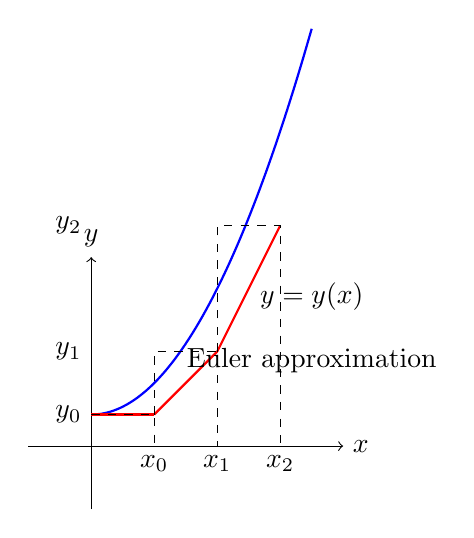
\begin{tikzpicture}[scale=0.8]
\draw[->] (-1,0) -- (4,0) node[right] {$x$};
\draw[->] (0,-1) -- (0,3) node[above] {$y$};
\draw[domain=0:3.5, smooth, variable=\x, blue, thick] plot ({\x}, {0.5*\x*\x + 0.5});
\draw[domain=0:1, smooth, variable=\x, red, thick] plot ({\x}, {0.5 + 0*\x});
\draw[domain=1:2, smooth, variable=\x, red, thick] plot ({\x}, {0.5 + 1*(\x-1)});
\draw[domain=2:3, smooth, variable=\x, red, thick] plot ({\x}, {1.5 + 2*(\x-2)});
\draw[dashed] (0,0.5) -- (1,0.5) -- (1,0);
\draw[dashed] (1,0.5) -- (1,1.5) -- (2,1.5) -- (2,0);
\draw[dashed] (2,1.5) -- (2,3.5) -- (3,3.5) -- (3,0);
\node[below] at (1,0) {$x_0$};
\node[below] at (2,0) {$x_1$};
\node[below] at (3,0) {$x_2$};
\node[left] at (0,0.5) {$y_0$};
\node[left] at (0,1.5) {$y_1$};
\node[left] at (0,3.5) {$y_2$};
\node[above] at (3.5,2) {$y = y(x)$};
\node[above] at (3.5,1) {Euler approximation};
\end{tikzpicture}
\end{center}

\textbf{Visual:}
\begin{itemize}
    \item Start at $(x_0, y_0)$
    \item Use slope $f(x_0, y_0)$ to step to next point
    \item Repeat process with new point
    \item Creates a piecewise linear approximation
\end{itemize}
\end{frame}

\begin{frame}{Euler's Method - Derivation}
\textbf{Step-by-step derivation:}
\begin{itemize}
    \item We have $\frac{dy}{dx} = f(x,y)$ and want to approximate $y(x)$
    \item At point $(x_n, y_n)$, the slope is $f(x_n, y_n)$
    \item Using linear approximation: $y(x_{n+1}) \approx y_n + f(x_n, y_n)(x_{n+1} - x_n)$
    \item Let $h = x_{n+1} - x_n$ (step size)
    \item Then: $y_{n+1} = y_n + h \cdot f(x_n, y_n)$
\end{itemize}
\end{frame}

\begin{frame}{Euler's Method - Formula}
\textbf{Euler's Method Formula:}
\[y_{n+1} = y_n + h \cdot f(x_n, y_n)\]
where $h$ is the step size and $x_{n+1} = x_n + h$

\textbf{Key Points:}
\begin{itemize}
    \item Requires the differential equation $\frac{dy}{dx} = f(x,y)$
    \item Need initial condition $y(x_0) = y_0$
    \item Choose step size $h$ (smaller = more accurate but more steps)
    \item Error accumulates with each step
    \item Simple but can be inaccurate for large step sizes
\end{itemize}
\end{frame}

\begin{frame}{Example 7: Euler's Method for Simple ODE}
\textbf{Problem:} Use Euler's Method to approximate the solution of $\frac{dy}{dx} = x + y$ with $y(0) = 1$ at $x = 0.5$ using step size $h = 0.1$

\textbf{Think about:}
\begin{itemize}
    \item What is your initial condition?
    \item How many steps do you need?
    \item What is $f(x,y)$ in this case?
    \item How do you calculate each step?
\end{itemize}
\end{frame}

\begin{frame}{Example 7: Euler's Method for Simple ODE - Solution}
\textbf{Solution:}
\begin{itemize}
    \item $\frac{dy}{dx} = x + y$, so $f(x,y) = x + y$
    \item Initial condition: $x_0 = 0$, $y_0 = 1$
    \item Step size: $h = 0.1$
    \item Need 5 steps to reach $x = 0.5$
    \item Euler's formula: $y_{n+1} = y_n + 0.1(x_n + y_n)$
\end{itemize}
\end{frame}

\begin{frame}{Example 7: Euler's Method for Simple ODE - Solution (Continued)}
\textbf{Iterations:}
\begin{itemize}
    \item $x_0 = 0$, $y_0 = 1$
    \item $x_1 = 0.1$, $y_1 = 1 + 0.1(0 + 1) = 1.1$
    \item $x_2 = 0.2$, $y_2 = 1.1 + 0.1(0.1 + 1.1) = 1.1 + 0.12 = 1.22$
    \item $x_3 = 0.3$, $y_3 = 1.22 + 0.1(0.2 + 1.22) = 1.22 + 0.142 = 1.362$
    \item $x_4 = 0.4$, $y_4 = 1.362 + 0.1(0.3 + 1.362) = 1.362 + 0.1662 = 1.5282$
    \item $x_5 = 0.5$, $y_5 = 1.5282 + 0.1(0.4 + 1.5282) = 1.5282 + 0.19282 = 1.72102$
    \item Approximation: $y(0.5) \approx 1.721$
\end{itemize}
\end{frame}

\begin{frame}{Example 8: Euler's Method for Exponential Growth}
\textbf{Problem:} Use Euler's Method to approximate the solution of $\frac{dy}{dx} = y$ with $y(0) = 1$ at $x = 1$ using step size $h = 0.25$

\textbf{Think about:}
\begin{itemize}
    \item What is the exact solution to this differential equation?
    \item How many steps do you need?
    \item How accurate do you expect the approximation to be?
\end{itemize}
\end{frame}

\begin{frame}{Example 8: Euler's Method for Exponential Growth - Solution}
\textbf{Solution:}
\begin{itemize}
    \item $\frac{dy}{dx} = y$, so $f(x,y) = y$
    \item Initial condition: $x_0 = 0$, $y_0 = 1$
    \item Step size: $h = 0.25$
    \item Need 4 steps to reach $x = 1$
    \item Euler's formula: $y_{n+1} = y_n + 0.25y_n = 1.25y_n$
\end{itemize}
\end{frame}

\begin{frame}{Example 8: Euler's Method for Exponential Growth - Solution (Continued)}
\textbf{Iterations:}
\begin{itemize}
    \item $x_0 = 0$, $y_0 = 1$
    \item $x_1 = 0.25$, $y_1 = 1.25 \times 1 = 1.25$
    \item $x_2 = 0.5$, $y_2 = 1.25 \times 1.25 = 1.5625$
    \item $x_3 = 0.75$, $y_3 = 1.25 \times 1.5625 = 1.953125$
    \item $x_4 = 1.0$, $y_4 = 1.25 \times 1.953125 = 2.441406$
    \item Approximation: $y(1) \approx 2.441$
    \item Exact solution: $y(x) = e^x$, so $y(1) = e \approx 2.718$
    \item Error: $|2.718 - 2.441| = 0.277$ (about 10\% error)
\end{itemize}
\end{frame}

\section{Error Analysis}

\begin{frame}{Newton's Method - Error Analysis}
\begin{itemize}
    \item Newton's Method has quadratic convergence
    \item If $r$ is the exact root, then $|x_{n+1} - r| \approx C|x_n - r|^2$
    \item This means the number of correct digits roughly doubles each iteration
    \item Method fails if:
    \begin{itemize}
        \item $f'(x_n) = 0$ (horizontal tangent)
        \item Initial guess is too far from root
        \item Function has multiple roots close together
    \end{itemize}
\end{itemize}
\end{frame}

\begin{frame}{Euler's Method - Error Analysis}
\begin{itemize}
    \item Euler's Method has linear convergence
    \item Local truncation error: $O(h^2)$ per step
    \item Global truncation error: $O(h)$ over the entire interval
    \item Error accumulates with each step
    \item Can be improved by:
    \begin{itemize}
        \item Using smaller step size
        \item Using more sophisticated methods (Runge-Kutta)
        \item Using adaptive step sizes
    \end{itemize}
\end{itemize}
\end{frame}

\section{Practice Problems}

\begin{frame}{Practice Problem 1}
\textbf{Problem:} Use Newton's Method to approximate $\sqrt{7}$ starting with $x_0 = 2.5$

\textbf{Hint:} Solve $x^2 = 7$ using $f(x) = x^2 - 7$.

\vspace{1cm}
\textbf{Steps to follow:}
\begin{enumerate}
    \item Write down the function $f(x)$ and its derivative $f'(x)$
    \item Write the Newton's Method formula
    \item Perform the iterations step by step
    \item Check your answer
\end{enumerate}
\end{frame}

\begin{frame}{Practice Problem 2}
\textbf{Problem:} Use Newton's Method to find a root of $f(x) = x^3 - x - 1$ starting with $x_0 = 1$

\textbf{Hint:} Calculate $f'(x) = 3x^2 - 1$ and use the Newton formula.

\vspace{1cm}
\textbf{Steps to follow:}
\begin{enumerate}
    \item Write down the function $f(x)$ and its derivative $f'(x)$
    \item Write the Newton's Method formula
    \item Perform the iterations step by step
    \item Check your answer by evaluating $f(x)$ at your final result
\end{enumerate}
\end{frame}

\begin{frame}{Practice Problem 3}
\textbf{Problem:} Use Euler's Method to approximate the solution of $\frac{dy}{dx} = 2x$ with $y(0) = 0$ at $x = 1$ using $h = 0.2$

\textbf{Hint:} This is a simple integration problem. What should the exact solution be?

\vspace{1cm}
\textbf{Steps to follow:}
\begin{enumerate}
    \item Identify $f(x,y)$ from the differential equation
    \item Determine how many steps you need
    \item Use Euler's formula: $y_{n+1} = y_n + h \cdot f(x_n, y_n)$
    \item Calculate each step carefully
    \item Compare with the exact solution
\end{enumerate}
\end{frame}

\begin{frame}{Practice Problem 4}
\textbf{Problem:} Use Euler's Method to approximate the solution of $\frac{dy}{dx} = -y$ with $y(0) = 1$ at $x = 1$ using $h = 0.25$

\textbf{Hint:} This is exponential decay. The exact solution is $y(x) = e^{-x}$.

\vspace{1cm}
\textbf{Steps to follow:}
\begin{enumerate}
    \item Identify $f(x,y)$ from the differential equation
    \item Determine how many steps you need
    \item Use Euler's formula: $y_{n+1} = y_n + h \cdot f(x_n, y_n)$
    \item Calculate each step carefully
    \item Compare with the exact solution $y(x) = e^{-x}$
\end{enumerate}
\end{frame}

\begin{frame}{Practice Problem 5}
\textbf{Problem:} Use Newton's Method to find a root of $f(x) = \cos(x) - x$ starting with $x_0 = 0.5$

\textbf{Hint:} You'll need to calculate $f'(x) = -\sin(x) - 1$.

\vspace{1cm}
\textbf{Steps to follow:}
\begin{enumerate}
    \item Write down the function $f(x)$ and its derivative $f'(x)$
    \item Write the Newton's Method formula
    \item Perform the iterations step by step
    \item Check your answer by evaluating $f(x)$ at your final result
\end{enumerate}
\end{frame}

\begin{frame}{Practice Problem 6}
\textbf{Problem:} Use Euler's Method to approximate the solution of $\frac{dy}{dx} = x^2 + y$ with $y(0) = 1$ at $x = 0.5$ using $h = 0.1$

\textbf{Hint:} This is a more complex ODE. Use the Euler formula carefully.

\vspace{1cm}
\textbf{Steps to follow:}
\begin{enumerate}
    \item Identify $f(x,y)$ from the differential equation
    \item Determine how many steps you need
    \item Use Euler's formula: $y_{n+1} = y_n + h \cdot f(x_n, y_n)$
    \item Calculate each step carefully, paying attention to both $x_n^2$ and $y_n$ terms
\end{enumerate}
\end{frame}

\begin{frame}{Practice Problem 7}
\textbf{Problem:} Use Newton's Method to find a root of $f(x) = e^x - 2x - 1$ starting with $x_0 = 1$

\textbf{Hint:} Calculate $f'(x) = e^x - 2$ and use the Newton formula.

\vspace{1cm}
\textbf{Steps to follow:}
\begin{enumerate}
    \item Write down the function $f(x)$ and its derivative $f'(x)$
    \item Write the Newton's Method formula
    \item Perform the iterations step by step
    \item Check your answer by evaluating $f(x)$ at your final result
\end{enumerate}
\end{frame}

\begin{frame}{Practice Problem 8}
\textbf{Problem:} Use Newton's Method to approximate $\sqrt[3]{10}$ starting with $x_0 = 2$

\textbf{Hint:} Solve $x^3 = 10$ using $f(x) = x^3 - 10$.

\vspace{1cm}
\textbf{Steps to follow:}
\begin{enumerate}
    \item Write down the function $f(x)$ and its derivative $f'(x)$
    \item Write the Newton's Method formula
    \item Perform the iterations step by step
    \item Check your answer by cubing your final result
\end{enumerate}
\end{frame}

\section{Solutions to Practice Problems}

\begin{frame}{Practice Problem 1 - Solution}
\textbf{Solution:} Approximate $\sqrt{7}$ using Newton's Method

\begin{itemize}
    \item $f(x) = x^2 - 7$, $f'(x) = 2x$
    \item Newton's formula: $x_{n+1} = x_n - \frac{x_n^2 - 7}{2x_n} = \frac{x_n + \frac{7}{x_n}}{2}$
    \item $x_0 = 2.5$
    \item $x_1 = \frac{2.5 + \frac{7}{2.5}}{2} = \frac{2.5 + 2.8}{2} = 2.65$
    \item $x_2 = \frac{2.65 + \frac{7}{2.65}}{2} = \frac{2.65 + 2.6415}{2} = 2.64575$
    \item $x_3 = \frac{2.64575 + \frac{7}{2.64575}}{2} = 2.645751$
    \item $\sqrt{7} \approx 2.645751$ (very accurate!)
\end{itemize}
\end{frame}

\begin{frame}{Practice Problem 2 - Solution}
\textbf{Solution:} Find root of $f(x) = x^3 - x - 1$ using Newton's Method

\begin{itemize}
    \item $f(x) = x^3 - x - 1$, $f'(x) = 3x^2 - 1$
    \item Newton's formula: $x_{n+1} = x_n - \frac{x_n^3 - x_n - 1}{3x_n^2 - 1}$
    \item $x_0 = 1$
    \item $x_1 = 1 - \frac{1 - 1 - 1}{3 - 1} = 1 - \frac{-1}{2} = 1.5$
    \item $x_2 = 1.5 - \frac{3.375 - 1.5 - 1}{6.75 - 1} = 1.5 - \frac{0.875}{5.75} = 1.3478$
    \item $x_3 = 1.3478 - \frac{2.448 - 1.3478 - 1}{5.45 - 1} = 1.3478 - \frac{0.1002}{4.45} = 1.3252$
    \item Root $\approx 1.3252$
\end{itemize}
\end{frame}

\begin{frame}{Practice Problem 3 - Solution}
\textbf{Solution:} Euler's Method for $\frac{dy}{dx} = 2x$ with $y(0) = 0$

\begin{itemize}
    \item $f(x,y) = 2x$, $h = 0.2$, need 5 steps to reach $x = 1$
    \item $x_0 = 0$, $y_0 = 0$
    \item $x_1 = 0.2$, $y_1 = 0 + 0.2(2 \times 0) = 0$
    \item $x_2 = 0.4$, $y_2 = 0 + 0.2(2 \times 0.2) = 0.08$
    \item $x_3 = 0.6$, $y_3 = 0.08 + 0.2(2 \times 0.4) = 0.08 + 0.16 = 0.24$
    \item $x_4 = 0.8$, $y_4 = 0.24 + 0.2(2 \times 0.6) = 0.24 + 0.24 = 0.48$
    \item $x_5 = 1.0$, $y_5 = 0.48 + 0.2(2 \times 0.8) = 0.48 + 0.32 = 0.80$
    \item Approximation: $y(1) \approx 0.80$
    \item Exact solution: $y(x) = x^2$, so $y(1) = 1$
    \item Error: $|1 - 0.80| = 0.20$ (20\% error)
\end{itemize}
\end{frame}

\begin{frame}{Practice Problem 4 - Solution}
\textbf{Solution:} Euler's Method for $\frac{dy}{dx} = -y$ with $y(0) = 1$

\begin{itemize}
    \item $f(x,y) = -y$, $h = 0.25$, need 4 steps to reach $x = 1$
    \item $x_0 = 0$, $y_0 = 1$
    \item $x_1 = 0.25$, $y_1 = 1 + 0.25(-1) = 0.75$
    \item $x_2 = 0.5$, $y_2 = 0.75 + 0.25(-0.75) = 0.75 - 0.1875 = 0.5625$
    \item $x_3 = 0.75$, $y_3 = 0.5625 + 0.25(-0.5625) = 0.5625 - 0.1406 = 0.4219$
    \item $x_4 = 1.0$, $y_4 = 0.4219 + 0.25(-0.4219) = 0.4219 - 0.1055 = 0.3164$
    \item Approximation: $y(1) \approx 0.3164$
    \item Exact solution: $y(x) = e^{-x}$, so $y(1) = e^{-1} \approx 0.3679$
    \item Error: $|0.3679 - 0.3164| = 0.0515$ (about 14\% error)
\end{itemize}
\end{frame}

\begin{frame}{Practice Problem 5 - Solution}
\textbf{Solution:} Find root of $f(x) = \cos(x) - x$ using Newton's Method

\begin{itemize}
    \item $f(x) = \cos(x) - x$, $f'(x) = -\sin(x) - 1$
    \item Newton's formula: $x_{n+1} = x_n - \frac{\cos(x_n) - x_n}{-\sin(x_n) - 1}$
    \item $x_0 = 0.5$
    \item $x_1 = 0.5 - \frac{\cos(0.5) - 0.5}{-\sin(0.5) - 1} = 0.5 - \frac{0.8776 - 0.5}{-0.4794 - 1} = 0.5 - \frac{0.3776}{-1.4794} = 0.7552$
    \item $x_2 = 0.7552 - \frac{\cos(0.7552) - 0.7552}{-\sin(0.7552) - 1} = 0.7552 - \frac{0.7281 - 0.7552}{-0.6845 - 1} = 0.7552 - \frac{-0.0271}{-1.6845} = 0.7391$
    \item $x_3 = 0.7391 - \frac{\cos(0.7391) - 0.7391}{-\sin(0.7391) - 1} = 0.7391 - \frac{0.7396 - 0.7391}{-0.6736 - 1} = 0.7391 - \frac{0.0005}{-1.6736} = 0.7391$
    \item Root $\approx 0.7391$ (this is a fixed point of $\cos(x)$)
\end{itemize}
\end{frame}

\begin{frame}{Practice Problem 6 - Solution}
\textbf{Solution:} Euler's Method for $\frac{dy}{dx} = x^2 + y$ with $y(0) = 1$

\begin{itemize}
    \item $f(x,y) = x^2 + y$, $h = 0.1$, need 5 steps to reach $x = 0.5$
    \item $x_0 = 0$, $y_0 = 1$
    \item $x_1 = 0.1$, $y_1 = 1 + 0.1(0^2 + 1) = 1 + 0.1 = 1.1$
    \item $x_2 = 0.2$, $y_2 = 1.1 + 0.1(0.1^2 + 1.1) = 1.1 + 0.1(0.01 + 1.1) = 1.1 + 0.111 = 1.211$
    \item $x_3 = 0.3$, $y_3 = 1.211 + 0.1(0.2^2 + 1.211) = 1.211 + 0.1(0.04 + 1.211) = 1.211 + 0.1251 = 1.3361$
    \item $x_4 = 0.4$, $y_4 = 1.3361 + 0.1(0.3^2 + 1.3361) = 1.3361 + 0.1(0.09 + 1.3361) = 1.3361 + 0.14261 = 1.47871$
    \item $x_5 = 0.5$, $y_5 = 1.47871 + 0.1(0.4^2 + 1.47871) = 1.47871 + 0.1(0.16 + 1.47871) = 1.47871 + 0.163871 = 1.642581$
    \item Approximation: $y(0.5) \approx 1.643$
\end{itemize}
\end{frame}

\begin{frame}{Practice Problem 7 - Solution}
\textbf{Solution:} Find root of $f(x) = e^x - 2x - 1$ using Newton's Method

\begin{itemize}
    \item $f(x) = e^x - 2x - 1$, $f'(x) = e^x - 2$
    \item Newton's formula: $x_{n+1} = x_n - \frac{e^{x_n} - 2x_n - 1}{e^{x_n} - 2}$
    \item $x_0 = 1$
    \item $x_1 = 1 - \frac{e^1 - 2(1) - 1}{e^1 - 2} = 1 - \frac{2.718 - 2 - 1}{2.718 - 2} = 1 - \frac{-0.282}{0.718} = 1.393$
    \item $x_2 = 1.393 - \frac{e^{1.393} - 2(1.393) - 1}{e^{1.393} - 2} = 1.393 - \frac{4.027 - 2.786 - 1}{4.027 - 2} = 1.393 - \frac{0.241}{2.027} = 1.274$
    \item $x_3 = 1.274 - \frac{e^{1.274} - 2(1.274) - 1}{e^{1.274} - 2} = 1.274 - \frac{3.575 - 2.548 - 1}{3.575 - 2} = 1.274 - \frac{0.027}{1.575} = 1.257$
    \item Root $\approx 1.257$
\end{itemize}
\end{frame}

\begin{frame}{Practice Problem 8 - Solution}
\textbf{Solution:} Approximate $\sqrt[3]{10}$ using Newton's Method

\begin{itemize}
    \item $f(x) = x^3 - 10$, $f'(x) = 3x^2$
    \item Newton's formula: $x_{n+1} = x_n - \frac{x_n^3 - 10}{3x_n^2} = x_n - \frac{x_n^3 - 10}{3x_n^2}$
    \item $x_0 = 2$
    \item $x_1 = 2 - \frac{8 - 10}{12} = 2 - \frac{-2}{12} = 2 + 0.167 = 2.167$
    \item $x_2 = 2.167 - \frac{10.18 - 10}{14.08} = 2.167 - \frac{0.18}{14.08} = 2.167 - 0.013 = 2.154$
    \item $x_3 = 2.154 - \frac{10.00 - 10}{13.92} = 2.154 - \frac{0.00}{13.92} = 2.154$
    \item $\sqrt[3]{10} \approx 2.154$ (very accurate!)
\end{itemize}
\end{frame}

\begin{frame}{Summary}
\begin{itemize}
    \item Newton's Method: $x_{n+1} = x_n - \frac{f(x_n)}{f'(x_n)}$ for finding roots
    \item Euler's Method: $y_{n+1} = y_n + h \cdot f(x_n, y_n)$ for solving ODEs
    \item Newton's Method has quadratic convergence (very fast)
    \item Euler's Method has linear convergence (slower, accumulates error)
    \item Both methods require good initial conditions
    \item Error analysis helps understand accuracy and limitations
    \item Newton's Method can fail with poor initial guesses
    \item Euler's Method accuracy improves with smaller step sizes
\end{itemize}
\end{frame}

\begin{frame}{Thank You!}
\centering
\vspace{2cm}
{\Huge \textcolor{myblue}{\textbf{Questions?}}}

\vspace{1cm}
{\Large Numerical methods are essential tools in modern mathematics and science!}
\end{frame}

\end{document} 